\documentclass[12pt,a4paper]{ctexart}
\usepackage[a4paper,margin=2.2cm]{geometry}
\usepackage{amsmath,amssymb}
\usepackage{booktabs}
\usepackage{longtable}
\usepackage{array}
\usepackage{graphicx}
\usepackage{float}
\usepackage{hyperref}
\usepackage{xcolor}
\usepackage{caption}
\usepackage{enumitem}
\graphicspath{{report_figures/}}

\hypersetup{
    colorlinks=true,
    linkcolor=blue,
    urlcolor=blue,
    citecolor=blue
}

\title{Lasso 回归优化实验报告\\
\large 基于 Subgradient、ISTA、FISTA 与 ADMM 的比较研究}
\author{最优化课程小组}
\date{\today}

\begin{document}
\maketitle

\begin{abstract}
本文围绕 Lasso 回归中的优化求解问题展开，比较了 Subgradient Descent、ISTA、FISTA 和 ADMM 四种算法在稀疏恢复任务中的表现。最终统一重跑以合成数据为主线，系统考察了基础对比、正则化参数 $\lambda$、ADMM 参数 $\rho$、重复实验稳定性和 \texttt{sklearn Lasso} 对照；同时在 \texttt{diabetes}、\texttt{wine\_red} 和 \texttt{Communities and Crime} 三个真实数据集上验证预测性能与收敛效率。早期完成的噪声、规模扩展、正则化路径与相变分析作为补充实验保留。结果表明：ISTA、FISTA 与 ADMM 能得到高度一致的解，其中 ADMM 通常需要更少迭代次数；$\lambda$ 控制误差与稀疏度之间的权衡，$\rho$ 则主要影响 ADMM 的收敛速度。
\end{abstract}

\section{课题背景与研究目标}
本课题围绕 Lasso 回归中的优化问题展开，重点比较以下四种算法在稀疏回归任务上的表现：
\begin{itemize}[leftmargin=2em]
    \item Subgradient Descent
    \item ISTA
    \item FISTA
    \item ADMM
\end{itemize}

Lasso 模型写作
\[
\min_x \frac{1}{2}\|Ax-b\|_2^2 + \lambda \|x\|_1
\]
其中，第一项刻画拟合误差，第二项通过 $L_1$ 正则诱导稀疏性。

本项目的研究目标包括：
\begin{enumerate}[label=\arabic*.]
    \item 在合成稀疏数据上比较四种算法的恢复误差、稀疏性和收敛速度；
    \item 分析正则化参数 $\lambda$ 与 ADMM 参数 $\rho$ 的影响；
    \item 分析噪声强度对稀疏恢复的影响；
    \item 在真实数据集上验证算法在实际回归任务中的预测表现；
    \item 通过正则化路径和相变分析补足 Lasso 主题下更完整的实验层次。
\end{enumerate}

\section{理论基础与算法原理}
\subsection{Lasso 模型的优化结构}
在高维回归中，常见情形是特征维度 $n$ 大于样本数 $m$。此时普通最小二乘问题可能出现解不唯一、模型不稳定和解释性较差等问题。Lasso 通过在最小二乘目标中引入 $L_1$ 正则项，鼓励得到稀疏解：
\[
\min_x \frac{1}{2}\|Ax-b\|_2^2 + \lambda \|x\|_1.
\]

该模型具有两个重要性质：
\begin{enumerate}[label=\arabic*.]
    \item 二次损失项 $\frac{1}{2}\|Ax-b\|_2^2$ 是凸且光滑可微的；
    \item 正则项 $\lambda \|x\|_1$ 是凸的，但在 $x_i=0$ 处不可微。
\end{enumerate}

因此，Lasso 是一个典型的\textbf{凸复合优化问题}，即
\[
\min_x f(x) + g(x),
\]
其中 $f(x)$ 光滑、$g(x)$ 非光滑但结构简单。也正因为这一结构，Lasso 不能直接依赖普通梯度下降，而更适合使用次梯度法、近端梯度法和 ADMM 等结构化优化方法。

进一步地，由于平方损失项与 $L_1$ 范数都为凸函数，Lasso 的整体目标函数也是凸的。这意味着本文比较的几种算法本质上是在求解同一个凸优化问题的全局最优解，只是它们利用问题结构的方式不同，因此在收敛路径、数值稳定性和计算效率上表现出明显差异。

\subsection{为什么 $L_1$ 正则能够诱导稀疏性}
与 $L_2$ 正则不同，$L_1$ 正则对应的近端算子具有“软阈值”形式：
\[
\mathrm{prox}_{\lambda \|\cdot\|_1}(v)
=
S_\lambda(v)
=
\mathrm{sign}(v)\max(|v|-\lambda,0).
\]
这个算子会把绝对值较小的分量直接压缩到 0，因此能够自然产生稀疏解。从优化角度看，Lasso 的稀疏性并不是“额外人工筛选”得到的，而是由 $L_1$ 正则的近端结构直接诱导出来的。这一点也解释了为什么在实验中，随着 $\lambda$ 增大，越来越多的特征系数会逐渐收缩为 0。

\subsection{Subgradient：直接处理非光滑项}
\subsection{Subgradient Descent}
对于不可微凸函数，可以使用次梯度替代普通梯度。Lasso 的一个次梯度可写为
\[
g(x)=A^\top(Ax-b)+\lambda s,\qquad s_i\in \partial |x_i|.
\]
其中，当 $x_i>0$ 时 $s_i=1$，当 $x_i<0$ 时 $s_i=-1$，当 $x_i=0$ 时 $s_i\in[-1,1]$。

因此，Subgradient 的更新形式为
\[
x^{k+1}=x^k-\alpha_k g(x^k).
\]

该方法的优点是实现简单、适用范围广；缺点是只利用局部次梯度信息，没有充分利用 Lasso 中 $L_1$ 项的特殊结构，因此通常收敛较慢，对步长也较为敏感。实验中观察到 Subgradient 的稀疏性和收敛速度都明显逊于其他三种结构化方法，这一现象与其理论特点一致。

\subsection{ISTA：近端梯度法}
\subsection{ISTA}
ISTA 适用于
\[
\min_x f(x)+g(x)
\]
这类复合优化问题，其中 $f$ 光滑且梯度 Lipschitz 连续，$g$ 非光滑但近端算子易于计算。

在 Lasso 中，有
\[
f(x)=\frac{1}{2}\|Ax-b\|_2^2,\qquad
g(x)=\lambda\|x\|_1,
\]
且
\[
\nabla f(x)=A^\top(Ax-b).
\]

由于 $\nabla f(x)$ 是线性的，其 Lipschitz 常数可以取为
\[
L=\|A^\top A\|_2.
\]
因此，在标准近端梯度理论中，步长通常满足
\[
0<t\le \frac{1}{L}.
\]
当步长满足这一条件时，ISTA 的更新具有标准的收敛保证。

ISTA 的更新公式为
\[
x^{k+1}
=
\mathrm{prox}_{t g}\bigl(x^k-t\nabla f(x^k)\bigr)
=
S_{t\lambda}\bigl(x^k-tA^\top(Ax^k-b)\bigr).
\]

因此，ISTA 的每一步都由“梯度下降 + 软阈值”组成，能够直接利用 $L_1$ 正则项的结构。理论上，ISTA 的目标函数收敛速度为 $O(1/k)$。

\subsection{FISTA：加速近端梯度法}
\subsection{FISTA}
FISTA 在 ISTA 基础上引入 Nesterov 动量项，通过在迭代中组合当前点和历史点来加速收敛。其理论目标函数收敛速度可提升到
\[
O(1/k^2),
\]
因此通常比 ISTA 更快。

更具体地说，FISTA 并没有改变 Lasso 问题本身，也没有改变软阈值近端映射；它的改进在于引入辅助序列和动量项，对 ISTA 的迭代轨迹进行加速。因此，FISTA 与 ISTA 共享相同的近端结构，但通过更积极地利用历史信息来获得更快的函数值下降。

需要注意的是，理论加速并不意味着在所有有限步实验中都一定出现大幅领先。实验中如果看到 FISTA 与 ISTA 的差距并不总是特别大，这往往与问题规模、停止准则以及参数设置有关；但从理论上看，FISTA 仍然是 ISTA 的自然加速版本。

\subsection{ADMM：变量分裂与增广拉格朗日}
\subsection{ADMM}
为了应用 ADMM，我们对 Lasso 做变量分裂：
\[
\min_{x,z}\frac{1}{2}\|Ax-b\|_2^2+\lambda\|z\|_1,
\qquad \text{s.t. } x=z.
\]

其增广拉格朗日函数为
\[
\mathcal{L}_\rho(x,z,u)
=
\frac{1}{2}\|Ax-b\|_2^2+\lambda\|z\|_1
+\frac{\rho}{2}\|x-z+u\|_2^2-\frac{\rho}{2}\|u\|_2^2.
\]

ADMM 的核心思想是交替更新：
\begin{enumerate}[label=\arabic*.]
    \item 固定 $z,u$，求解 $x$ 的二次子问题；
    \item 固定 $x,u$，对 $z$ 做软阈值更新；
    \item 更新对偶变量 $u$。
\end{enumerate}

对应的标准更新式可以写为：
\[
x^{k+1}
=
\arg\min_x
\frac{1}{2}\|Ax-b\|_2^2
+\frac{\rho}{2}\|x-z^k+u^k\|_2^2,
\]
\[
z^{k+1}
=
\arg\min_z
\lambda\|z\|_1
+\frac{\rho}{2}\|x^{k+1}-z+u^k\|_2^2,
\]
\[
u^{k+1}=u^k+x^{k+1}-z^{k+1}.
\]

其中，$x$ 子问题是一个二次优化问题，$z$ 子问题则仍然具有软阈值闭式解。因此，ADMM 的每一步都与 Lasso 的问题结构高度匹配。

这样一来，原问题被拆成“线性系统求解 + 软阈值”两个结构清晰的子问题，因此非常适合 Lasso 这类“光滑项 + 非光滑项”的组合优化问题。本项目中 ADMM 之所以表现突出，正是因为它充分利用了问题的结构，而不是把整个目标函数当作一般不可微问题处理。

\subsection{参数 $\lambda$ 与 $\rho$ 的理论作用}
正则化参数 $\lambda$ 控制拟合误差与稀疏性之间的平衡：
\begin{itemize}[leftmargin=2em]
    \item $\lambda$ 较小时，模型更倾向于拟合数据，解往往较稠密；
    \item $\lambda$ 较大时，软阈值效应更强，更多系数被压缩为 0，但也可能带来过度收缩。
\end{itemize}

ADMM 中的 $\rho$ 则是增广拉格朗日的惩罚参数，它主要影响收敛过程而不是最终最优解：
\begin{itemize}[leftmargin=2em]
    \item $\rho$ 过小时，约束 $x=z$ 的一致性推进较慢；
    \item $\rho$ 过大时，子问题可能变得更僵硬，数值上不利于快速收敛；
    \item 因此通常需要在中等范围内选择较合适的 $\rho$。
\end{itemize}

在 ADMM 的收敛监控中，常用原始残差与对偶残差分别衡量约束满足程度与对偶稳定性：
\[
r^k=x^k-z^k,\qquad s^k=\rho(z^k-z^{k-1}).
\]
其中，原始残差 $r^k$ 反映约束 $x=z$ 是否已基本满足；对偶残差 $s^k$ 则反映迭代过程中对偶变量所对应的变化是否已经稳定。因此，$\rho$ 的选择不仅影响每一步子问题的数值性质，也会直接影响这两类残差的衰减速度。

这也正是后续实验中需要分别分析 $\lambda$ 与 $\rho$ 的理论原因。

\section{数据集设置}
\subsection{合成数据}
合成数据用于主实验，因为真实稀疏解 $x^\ast$ 已知，可以直接评估：
\begin{itemize}[leftmargin=2em]
    \item 恢复误差 $\|\hat{x} - x^\ast\|_2$
    \item 非零元素个数
    \item 支撑集恢复是否成功
\end{itemize}

合成数据构造方式如下：
\begin{enumerate}[label=\arabic*.]
    \item 生成高斯随机矩阵 $A$；
    \item 按列归一化，减弱特征尺度不一致带来的影响；
    \item 生成稀疏真实信号 $x^\ast$，仅保留少数非零元素；
    \item 加入高斯噪声，构造观测 $b = Ax^\ast + \varepsilon$。
\end{enumerate}

\subsection{真实数据}
目前使用了三个真实回归数据集：
\begin{itemize}[leftmargin=2em]
    \item \texttt{diabetes}：来自 \texttt{sklearn}，规模较小，适合作为真实数据补充实验；
    \item \texttt{winequality-red.csv}：来自 UCI Wine Quality 数据集，使用红酒子集作为第二个真实数据验证场景。
    \item \texttt{Communities and Crime}：来自 UCI，存在缺失值，特征更多，适合作为复杂真实高维回归场景的补充实验。
\end{itemize}

\begin{center}
\begin{tabular}{lccc}
\toprule
数据集 & 训练集规模 & 测试集规模 & 特征数 \\
\midrule
diabetes & 353 & 89 & 10 \\
wine\_red & 1279 & 320 & 11 \\
Communities and Crime & 1595 & 399 & 100（清洗后） \\
\bottomrule
\end{tabular}
\end{center}

三个真实数据集均按 80\%/20\% 划分训练集和测试集，并且只使用训练集统计量完成特征与目标变量标准化。对于 Communities and Crime，还额外进行缺失列删除和中位数填补。更完整的数据集来源、预处理流程与实验设计统一记录在 \texttt{DATASETS\_AND\_EXPERIMENTS.md} 中。

原本尝试接入 \texttt{California Housing}，但运行中遇到远程下载的 HTTP 403 问题，因此最终采用了本地可控的 \texttt{wine\_red} 与 \texttt{Communities and Crime} 数据。

需要特别说明的是：合成数据与真实数据并不是做完全相同的实验，而是有明确分工：
\begin{itemize}[leftmargin=2em]
    \item \textbf{合成数据}：负责机制分析。因为知道真实稀疏解，所以可以做恢复误差、支撑集恢复、相变分析、噪声实验和规模扩展实验。
    \item \textbf{真实数据}：负责应用验证。因为真实数据中不知道真实系数，所以重点考察预测误差、稀疏性和收敛效率。
\end{itemize}

从理论上看，这种分工是自然的。合成数据满足“真实系数已知”的设定，因此可以讨论支持恢复是否成功；而真实数据中的真实回归系数通常未知，且数据本身未必严格满足一个稀疏线性真值模型，因此在真实数据上更合理的评价指标是训练误差、测试误差、非零特征个数以及算法收敛效率，而不是恢复误差或支持恢复正确率。

\section{实验实现中的修正与改进}
这一部分很重要，因为本项目并不是一次性得到完美结果，而是经历了“初版结果不理想 $\rightarrow$ 排查与修改 $\rightarrow$ 正式版结果”的过程。

\subsection{初版存在的问题}
\begin{enumerate}[label=\arabic*.]
    \item \textbf{Subgradient 在真实数据上出现数值不稳定。} 初版在 \texttt{diabetes} 上一度出现 \texttt{nan}。
    \item \textbf{日志中出现大量 RuntimeWarning。} 虽然很多结果数值本身正常，但日志不够干净，不适合后续汇报展示。
    \item \textbf{相变分析初版成功率全为 0。} 这使得“成功率曲线”本身不可解释。
    \item \textbf{中等规模主实验中，初始选取的 $\lambda=0.05$ 虽然误差较低，但解偏稠密，不利于展示 Lasso 的稀疏恢复特性。}
\end{enumerate}

\subsection{对应修正}
\begin{enumerate}[label=\arabic*.]
    \item 对 Subgradient 的步长做了 Lipschitz 尺度归一化，使其从“数值发散”调整为“可以运行但收敛慢的 baseline”。
    \item 对关键矩阵乘法加入安全封装，清理误导性警告。
    \item 最终统一重跑采用 $\lambda=0.1$，在恢复误差与稀疏度之间取得折中，并将所有结果集中保存到同一个时间戳目录。
    \item 相变分析新增两种成功标准：
    \begin{itemize}[leftmargin=2em]
        \item 严格标准：支撑集完全一致；
        \item 宽松标准：命中至少 80\% 的真实非零位置。
    \end{itemize}
    \item 相变分析还调整为更适合观察趋势的实验规模：$m=120, n=300, s=10$。
\end{enumerate}

\section{已完成实验总览}
到目前为止，已经完成以下实验：
\begin{enumerate}[label=\arabic*.]
    \item 小规模合成数据基线实验
    \item 最终统一重跑合成数据主实验
    \item $\lambda$ 敏感性分析
    \item $\rho$ 敏感性分析
    \item 噪声强度实验
    \item 多随机种子重复实验
    \item 三档规模对比实验
    \item 正则化路径可视化
    \item 相变分析（严格版与宽松版）
    \item 真实数据实验：\texttt{diabetes}
    \item 真实数据实验：\texttt{wine\_red}
    \item 真实数据实验：\texttt{Communities and Crime}
    \item \texttt{sklearn Lasso} 对照验证
\end{enumerate}

\section{最终统一重跑说明}
为保证报告、PPT 与提交结果完全一致，本文将
\texttt{results/final\_rerun\_20260606\_172023/}
作为最终结果来源。统一运行脚本为 \texttt{run\_final\_experiments.py}，每次运行均创建新的时间戳目录，不覆盖旧结果。最终统一重跑包含合成数据基础实验、$\lambda$ 敏感性、ADMM 的 $\rho$ 敏感性、五个随机种子重复实验、\texttt{sklearn Lasso} 对照，以及三个真实数据集实验。早期完成的噪声、规模扩展、正则化路径和相变分析作为补充实验保留，但不与最终统一重跑的数值表混用。

\section{实验一：合成数据基础实验}
\subsection{实验目的}
该实验用于：
\begin{itemize}[leftmargin=2em]
    \item 验证四种算法都能正常运行；
    \item 展示基础的收敛速度差异；
    \item 画出收敛曲线和系数恢复图。
\end{itemize}

\subsection{实验设置}
\begin{itemize}[leftmargin=2em]
    \item $m=80$
    \item $n=200$
    \item 稀疏度 $s=10$
    \item 噪声水平 $\sigma=0.05$
    \item $\lambda=0.1$
    \item $\rho=1$
    \item 最大迭代次数 500
\end{itemize}

\subsection{主要现象}
\begin{itemize}[leftmargin=2em]
    \item Subgradient 产生的解几乎不稀疏；
    \item ISTA、FISTA、ADMM 都能得到明显更稀疏的解；
    \item ADMM 的迭代次数显著少于其他方法。
\end{itemize}

\section{实验二：最终统一重跑主结果}
\subsection{实验目的}
该实验是本项目最核心的正式主实验，主要用于：
\begin{itemize}[leftmargin=2em]
    \item 在统一可复现设置下比较四种算法；
    \item 形成参数分析、重复实验和对照验证的统一主设置；
    \item 作为期末作业报告中的主结果来源。
\end{itemize}

\subsection{实验设置}
\begin{itemize}[leftmargin=2em]
    \item $m=80$
    \item $n=200$
    \item 稀疏度 $s=10$
    \item 噪声水平 $\sigma=0.05$
    \item $\lambda=0.1$
    \item $\rho=1$
    \item 最大迭代次数 500
\end{itemize}

\subsection{为什么统一重跑采用 $\lambda=0.1$}
统一重跑同时比较了多个 $\lambda$。结果表明：
\begin{itemize}[leftmargin=2em]
    \item $\lambda=0.05$ 时恢复误差最低，约为 0.343，但解保留约 36 个非零系数；
    \item $\lambda=0.1$ 时恢复误差约为 0.390，并将非零系数减少到 17；
    \item $\lambda=0.2$ 时仅保留 7 个非零系数，已出现较明显的过度收缩。
\end{itemize}
因此，最终统一重跑采用 $\lambda=0.1$，在恢复误差和稀疏度之间取得较平衡的结果。

\subsection{正式主实验结果}
\begin{center}
\begin{tabular}{lcccc}
\toprule
算法 & recovery\_error & nnz & iter & 备注 \\
\midrule
Subgradient & 0.424933 & 200 & 500 & 未产生严格稀疏解 \\
ISTA & 0.389504 & 17 & 176 & 稀疏恢复较好 \\
FISTA & 0.389507 & 17 & 168 & 与 ISTA 接近 \\
ADMM & 0.389504 & 17 & 59 & 迭代次数最少 \\
\bottomrule
\end{tabular}
\end{center}

\begin{figure}[H]
    \centering
    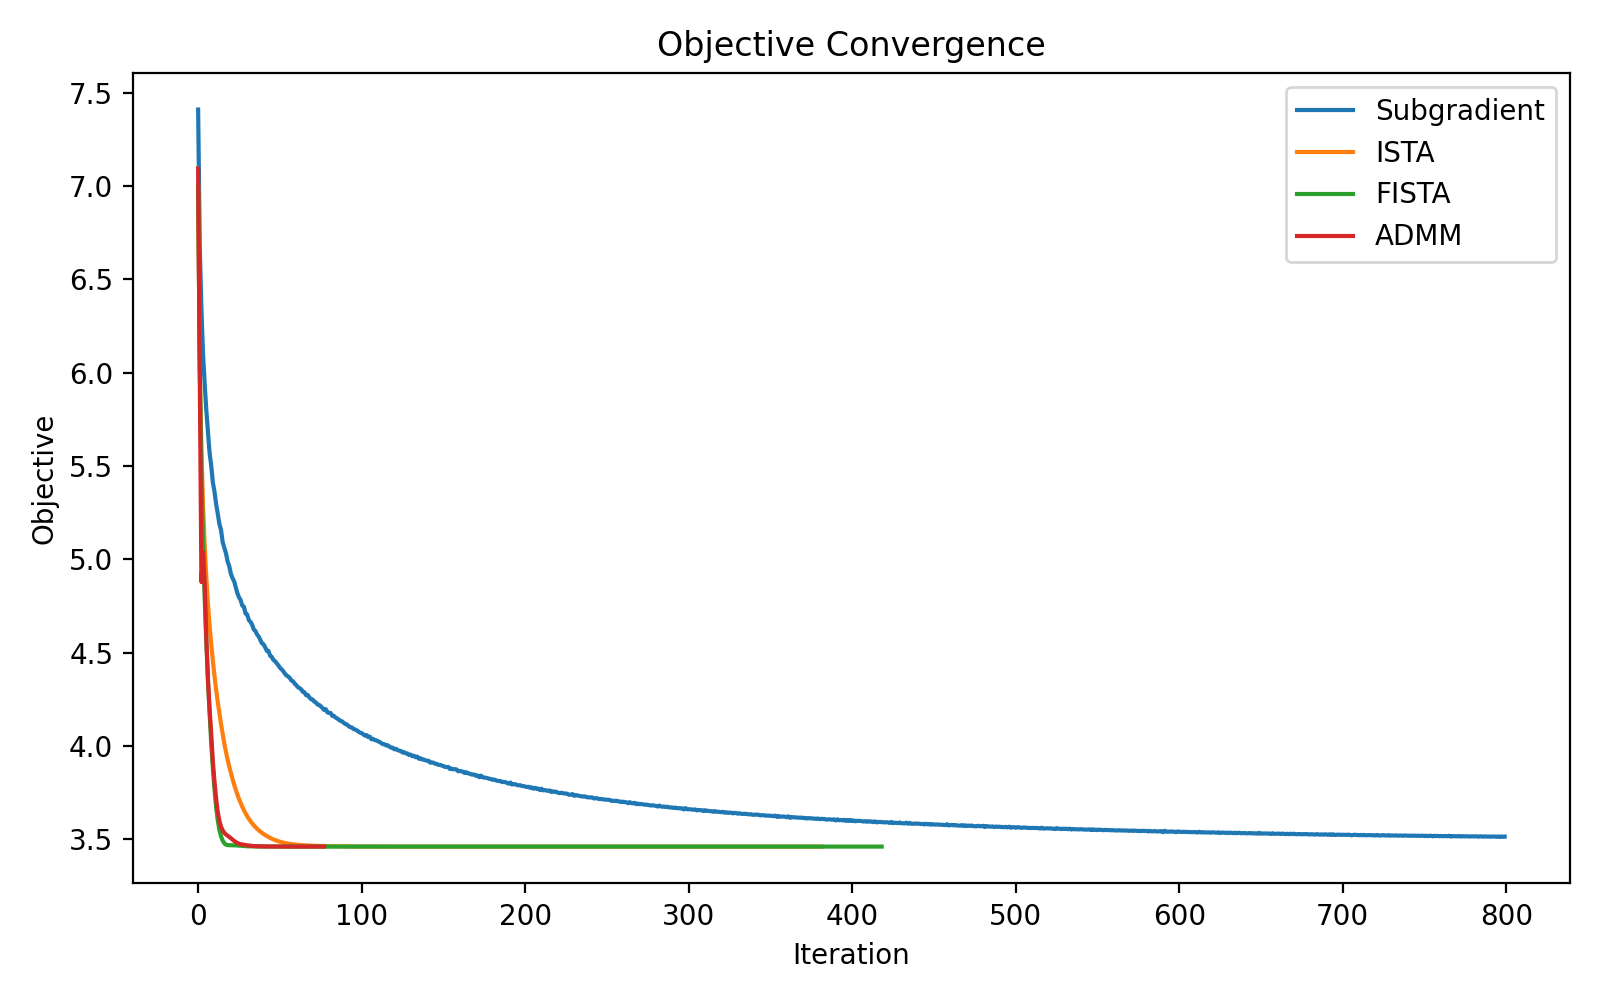
\includegraphics[width=0.82\textwidth]{01_synthetic_main_convergence_curve.png}
    \caption{最终统一重跑中合成数据主实验的收敛曲线。ISTA、FISTA 与 ADMM 收敛到几乎相同的目标值，其中 ADMM 迭代次数最少。}
\end{figure}

\begin{figure}[H]
    \centering
    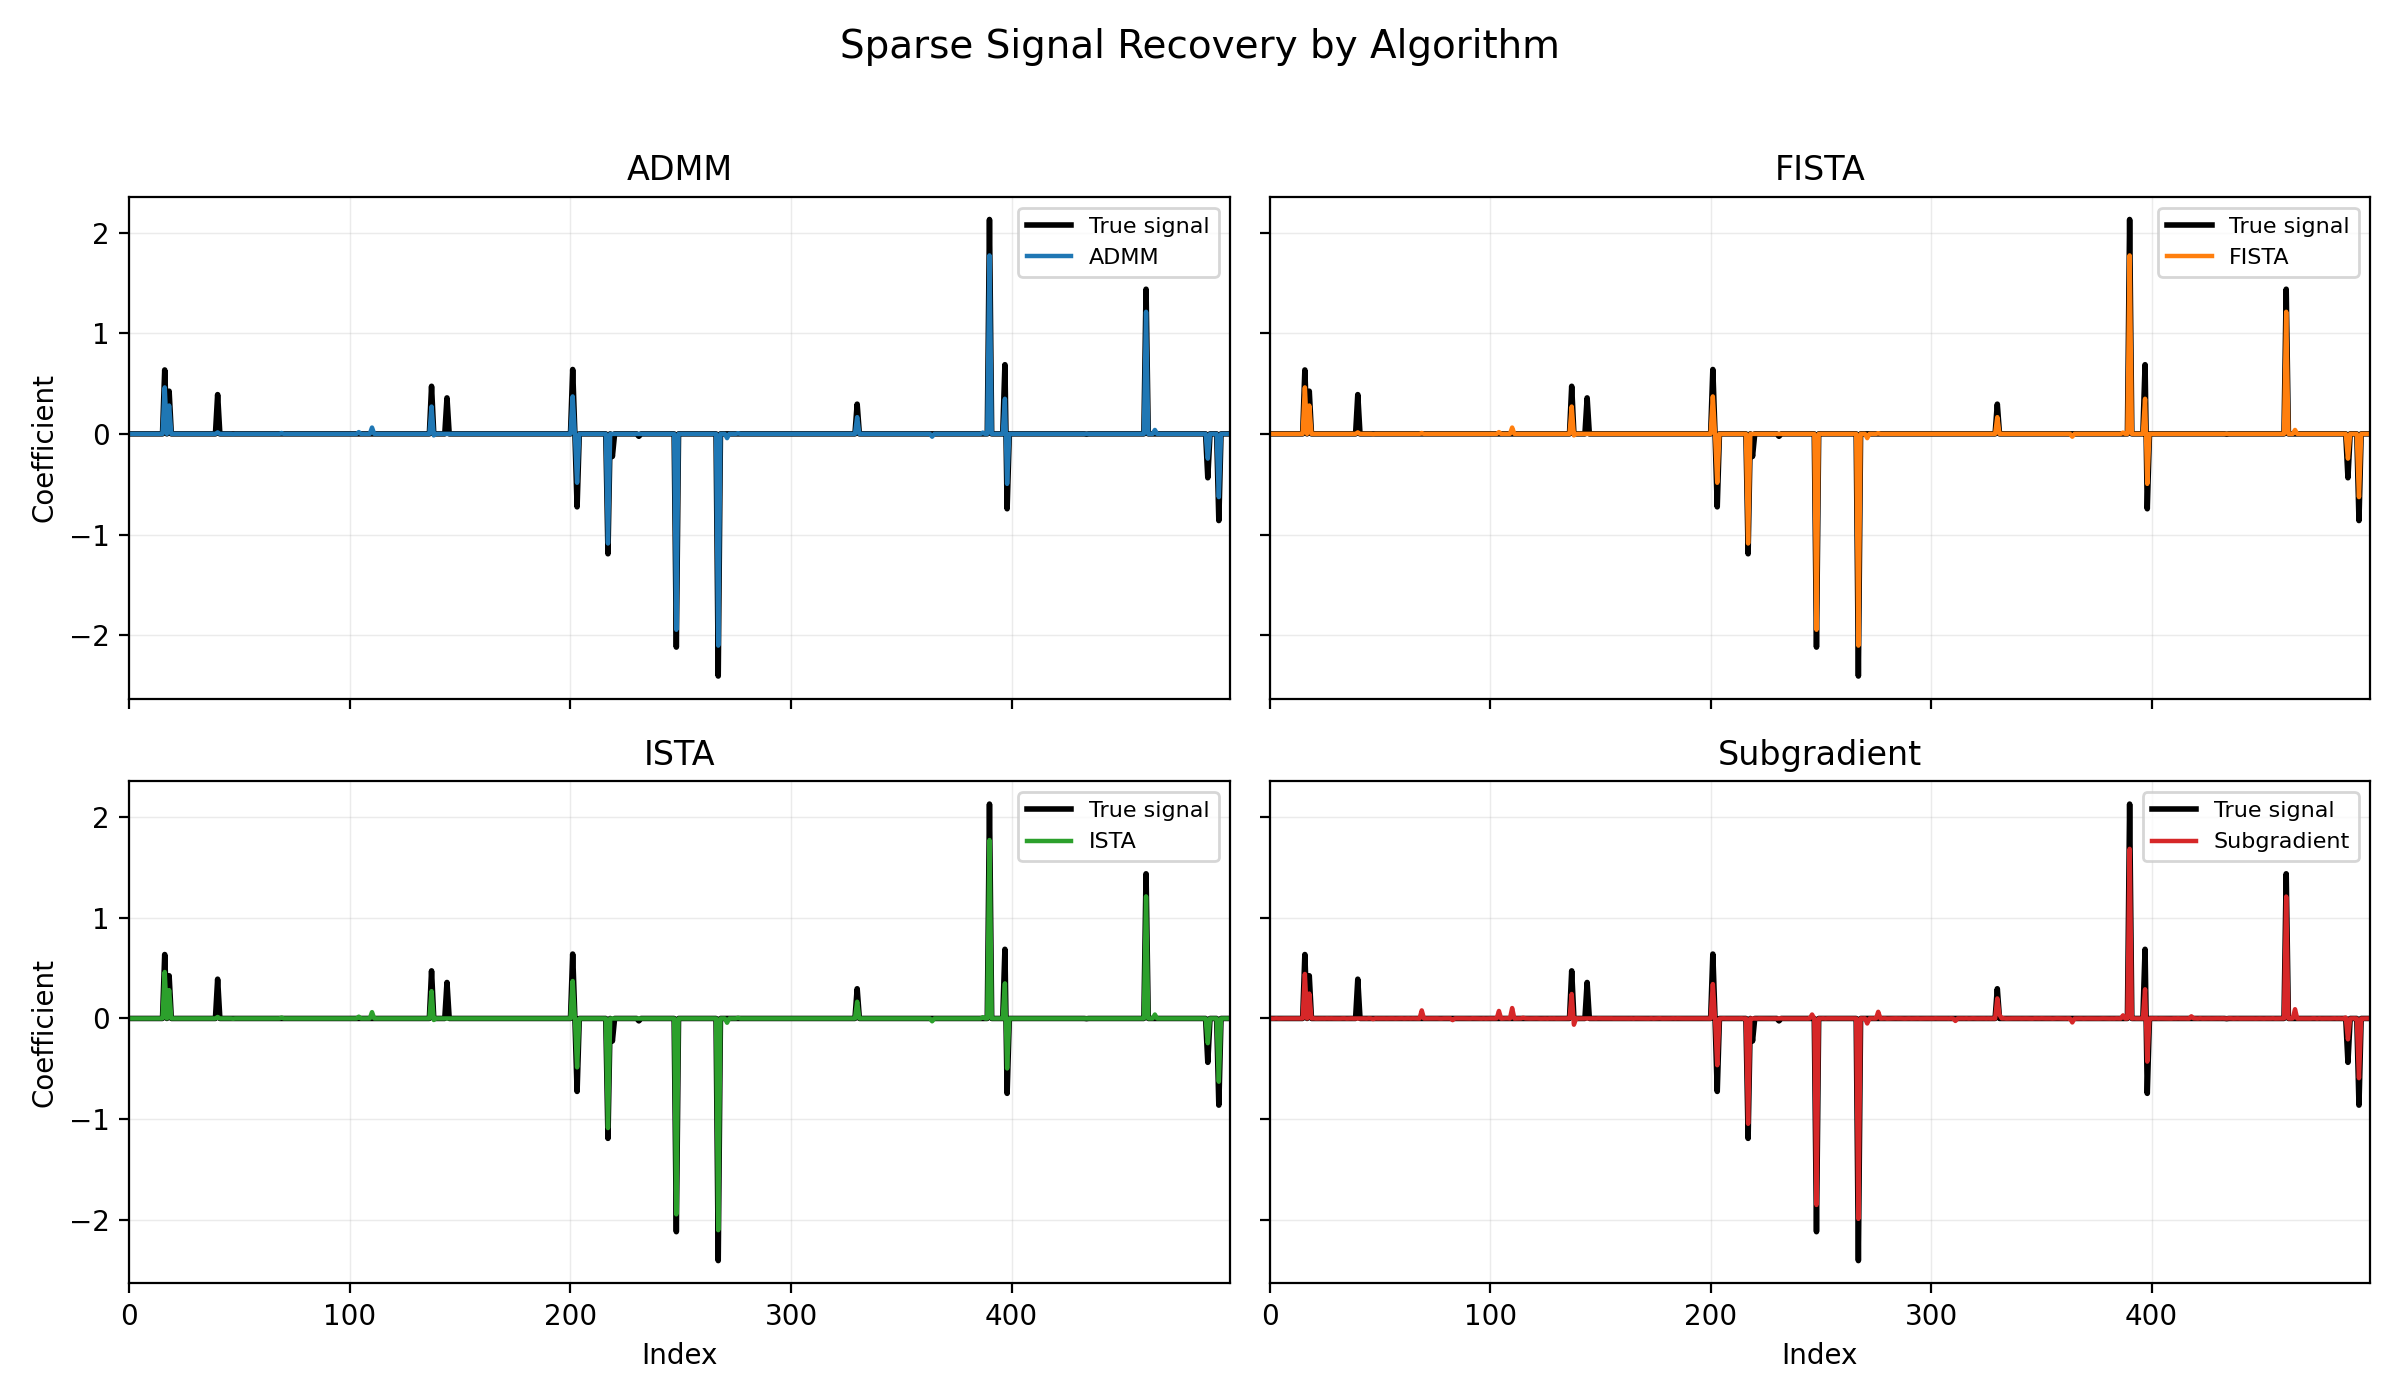
\includegraphics[width=0.82\textwidth]{02_synthetic_main_sparse_recovery_coefficients.png}
    \caption{最终统一重跑中的真实系数与恢复系数对比图。Subgradient 基本未产生严格稀疏解，而 ISTA、FISTA 和 ADMM 得到了高度一致的稀疏结果。}
\end{figure}

\subsection{结论}
\begin{enumerate}[label=\arabic*.]
    \item Subgradient 作为 baseline 效果最差，几乎无法产生理想稀疏解；
    \item ISTA、FISTA、ADMM 都能恢复出接近真实稀疏度的解；
    \item ADMM 在迭代次数上明显占优，是该设置下最突出的算法。
\end{enumerate}

\section{实验三：$\lambda$ 敏感性分析}
\subsection{实验目的}
研究正则化参数 $\lambda$ 对以下指标的影响：
\begin{itemize}[leftmargin=2em]
    \item 恢复误差
    \item 解的稀疏性
    \item 收敛速度
\end{itemize}

\subsection{实验设置}
固定最终统一重跑场景：
\begin{itemize}[leftmargin=2em]
    \item $m=80$
    \item $n=200$
    \item 稀疏度 $s=10$
    \item $\sigma=0.05$
    \item $\rho=1$
\end{itemize}
考察的 $\lambda$ 为：
\[
0.01,\ 0.02,\ 0.05,\ 0.1,\ 0.2,\ 0.5,\ 1.0
\]

\subsection{主要观察}
\begin{itemize}[leftmargin=2em]
    \item $\lambda=0.01$ 时解非常稠密；
    \item $\lambda=0.05$ 时恢复误差最低，约为 0.343，但非零个数为 36；
    \item $\lambda=0.1$ 时非零个数下降到 17，恢复误差约为 0.390；
    \item $\lambda=0.2$ 时非零个数下降到 7，开始出现过度收缩；
    \item $\lambda=1.0$ 时仅剩 2 个非零系数，恢复误差增大到约 1.561。
\end{itemize}

\subsection{结论}
该实验清楚展示了 Lasso 的核心权衡：较小的 $\lambda$ 利于降低恢复误差，较大的 $\lambda$ 会增强稀疏性但可能过度收缩。最终统一重跑采用 $\lambda=0.1$ 作为误差与稀疏度之间的折中。

\section{实验四：$\rho$ 敏感性分析}
\subsection{实验目的}
研究 ADMM 参数 $\rho$ 对收敛速度和最终结果的影响。

\subsection{实验设置}
\begin{itemize}[leftmargin=2em]
    \item $m=80$
    \item $n=200$
    \item $s=10$
    \item $\sigma=0.05$
    \item $\lambda=0.1$
    \item $\rho \in \{0.1, 0.5, 1, 2, 5, 10\}$
\end{itemize}

\subsection{主要结果}
\begin{center}
\begin{tabular}{lcc}
\toprule
$\rho$ & ADMM iter & 说明 \\
\midrule
0.1 & 500 & 未在最大迭代数内满足停止条件 \\
0.5 & 114 & 明显改善 \\
1 & 59 & 最快 \\
2 & 63 & 与 $\rho=1$ 接近 \\
5 & 172 & 再次变慢 \\
10 & 342 & 明显变慢 \\
\bottomrule
\end{tabular}
\end{center}

\subsection{结论}
不同 $\rho$ 下最终目标值、恢复误差和 nnz 几乎相同，但收敛速度差异显著。当前实验设置下，$\rho=1$ 最快，$\rho=2$ 也具有相近表现。

\section{补充实验一：噪声强度实验（早期扩展）}
\subsection{实验目的}
考察观测噪声水平对稀疏恢复难度的影响。

\subsection{实验设置}
\begin{itemize}[leftmargin=2em]
    \item $m=150$
    \item $n=500$
    \item $s=20$
    \item $\lambda=0.2$
    \item $\rho=1$
    \item $\sigma \in \{0.00, 0.01, 0.05, 0.10\}$
\end{itemize}

\subsection{主要结果}
以 ADMM 为例：
\begin{center}
\begin{tabular}{lcc}
\toprule
$\sigma$ & recovery\_error & nnz \\
\midrule
0.00 & 1.058223 & 17 \\
0.01 & 1.056204 & 19 \\
0.05 & 1.067471 & 26 \\
0.10 & 1.301248 & 50 \\
\bottomrule
\end{tabular}
\end{center}

\subsection{结论}
噪声越大，恢复误差越大，恢复出的解越不稀疏，说明噪声会显著破坏对真实稀疏结构的识别能力。

\section{实验六：多随机种子重复实验}
\subsection{实验目的}
前面的主实验大多基于单个随机种子。为了减少单次随机生成数据带来的偶然性，我们进一步在多个随机种子下重复主实验，并统计各指标的均值与标准差。

\subsection{实验设置}
\begin{itemize}[leftmargin=2em]
    \item 主实验参数保持不变：
    \begin{itemize}[leftmargin=2em]
        \item $m=80$
        \item $n=200$
        \item 稀疏度 $s=10$
        \item $\sigma=0.05$
        \item $\lambda=0.1$
        \item $\rho=1$
    \end{itemize}
    \item 随机种子取 $\{0,1,2,3,4\}$
    \item 记录指标：
    \begin{itemize}[leftmargin=2em]
        \item 恢复误差均值与标准差
        \item 非零元素个数均值与标准差
        \item 迭代次数均值与标准差
    \end{itemize}
\end{itemize}

\subsection{实验结果}
\begin{center}
\begin{tabular}{lccc}
\toprule
算法 & recovery\_error\_mean & nnz\_mean & iter\_mean \\
\midrule
ADMM & 0.371363 & 19.2 & 61.0 \\
FISTA & 0.371366 & 19.2 & 221.2 \\
ISTA & 0.371370 & 19.4 & 221.0 \\
Subgradient & 0.799093 & 200.0 & 500.0 \\
\bottomrule
\end{tabular}
\end{center}

\begin{figure}[H]
    \centering
    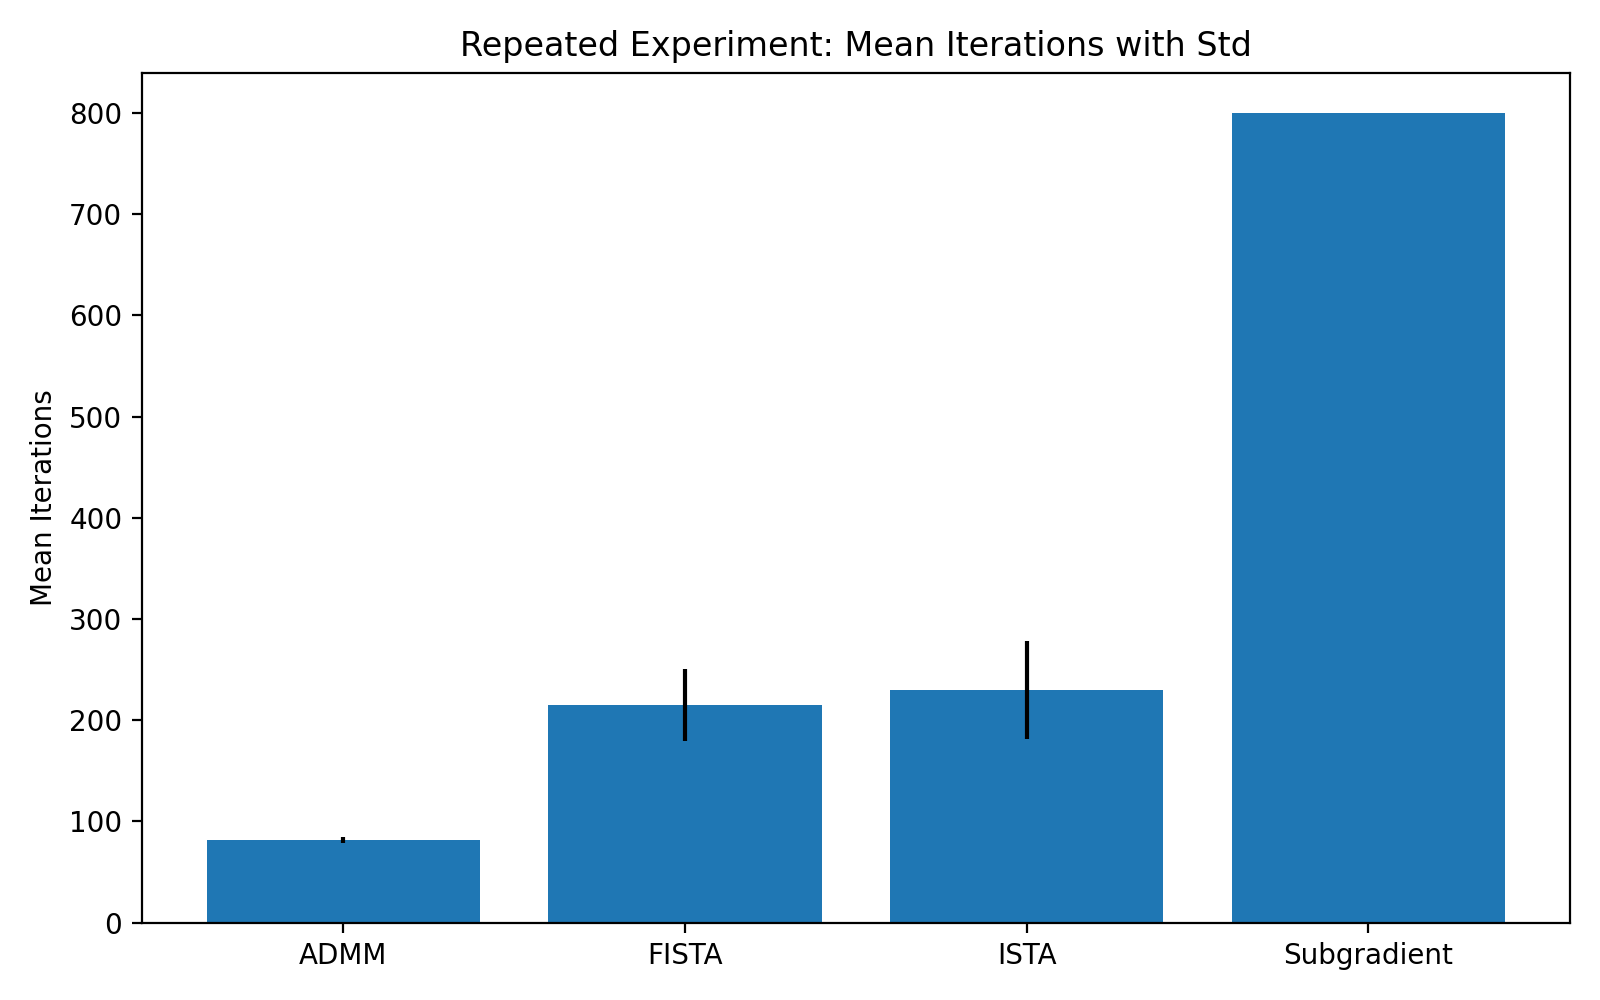
\includegraphics[width=0.72\textwidth]{03_repeat_experiment_mean_iterations.png}
    \caption{多随机种子重复实验下，各算法恢复误差对比。ISTA、FISTA 和 ADMM 的结果几乎重合，说明主实验结论并非单次随机实验的偶然现象。}
\end{figure}

\subsection{结果分析}
\begin{enumerate}[label=\arabic*.]
    \item ADMM、ISTA、FISTA 在恢复误差和稀疏度上都较为稳定，说明主实验结论不是偶然现象；
    \item ADMM 的平均迭代次数显著低于 ISTA 和 FISTA；
    \item Subgradient 即使在重复实验下仍然表现最差，说明其劣势是稳定存在的，而不是某一次随机实验造成的。
\end{enumerate}

\subsection{结论}
重复实验显著增强了结果的可信度，也使本项目从“单次演示实验”提升为“具有统计稳定性分析”的期末作业。

\section{补充实验二：三档规模对比实验（早期扩展）}
\subsection{实验目的}
研究问题规模增大时，各算法的恢复误差、稀疏性和收敛速度如何变化。相比只增大某一个参数，三档规模对比更能系统展示算法在高维场景下的适应性。

\subsection{实验设置}
固定：
\begin{itemize}[leftmargin=2em]
    \item $\sigma=0.05$
    \item $\lambda=0.2$
    \item $\rho=1$
\end{itemize}

三档规模分别为：
\begin{itemize}[leftmargin=2em]
    \item 小规模：$m=80,\ n=200,\ s=10$
    \item 中规模：$m=150,\ n=500,\ s=20$
    \item 大规模：$m=300,\ n=1000,\ s=30$
\end{itemize}

\subsection{实验结果}
\begin{center}
\begin{tabular}{llccc}
\toprule
规模 & 算法 & recovery\_error & nnz & iter \\
\midrule
80/200/10 & ADMM & 0.578516 & 7 & 70 \\
80/200/10 & ISTA & 0.578516 & 7 & 97 \\
80/200/10 & FISTA & 0.578516 & 7 & 117 \\
80/200/10 & Subgradient & 0.582503 & 200 & 800 \\
\midrule
150/500/20 & ADMM & 1.067471 & 26 & 80 \\
150/500/20 & ISTA & 1.067482 & 26 & 241 \\
150/500/20 & FISTA & 1.067467 & 26 & 254 \\
150/500/20 & Subgradient & 1.248809 & 499 & 800 \\
\midrule
300/1000/30 & ADMM & 1.235796 & 31 & 84 \\
300/1000/30 & ISTA & 1.235805 & 31 & 221 \\
300/1000/30 & FISTA & 1.235818 & 31 & 198 \\
300/1000/30 & Subgradient & 1.393068 & 1000 & 800 \\
\bottomrule
\end{tabular}
\end{center}

\begin{figure}[H]
    \centering
    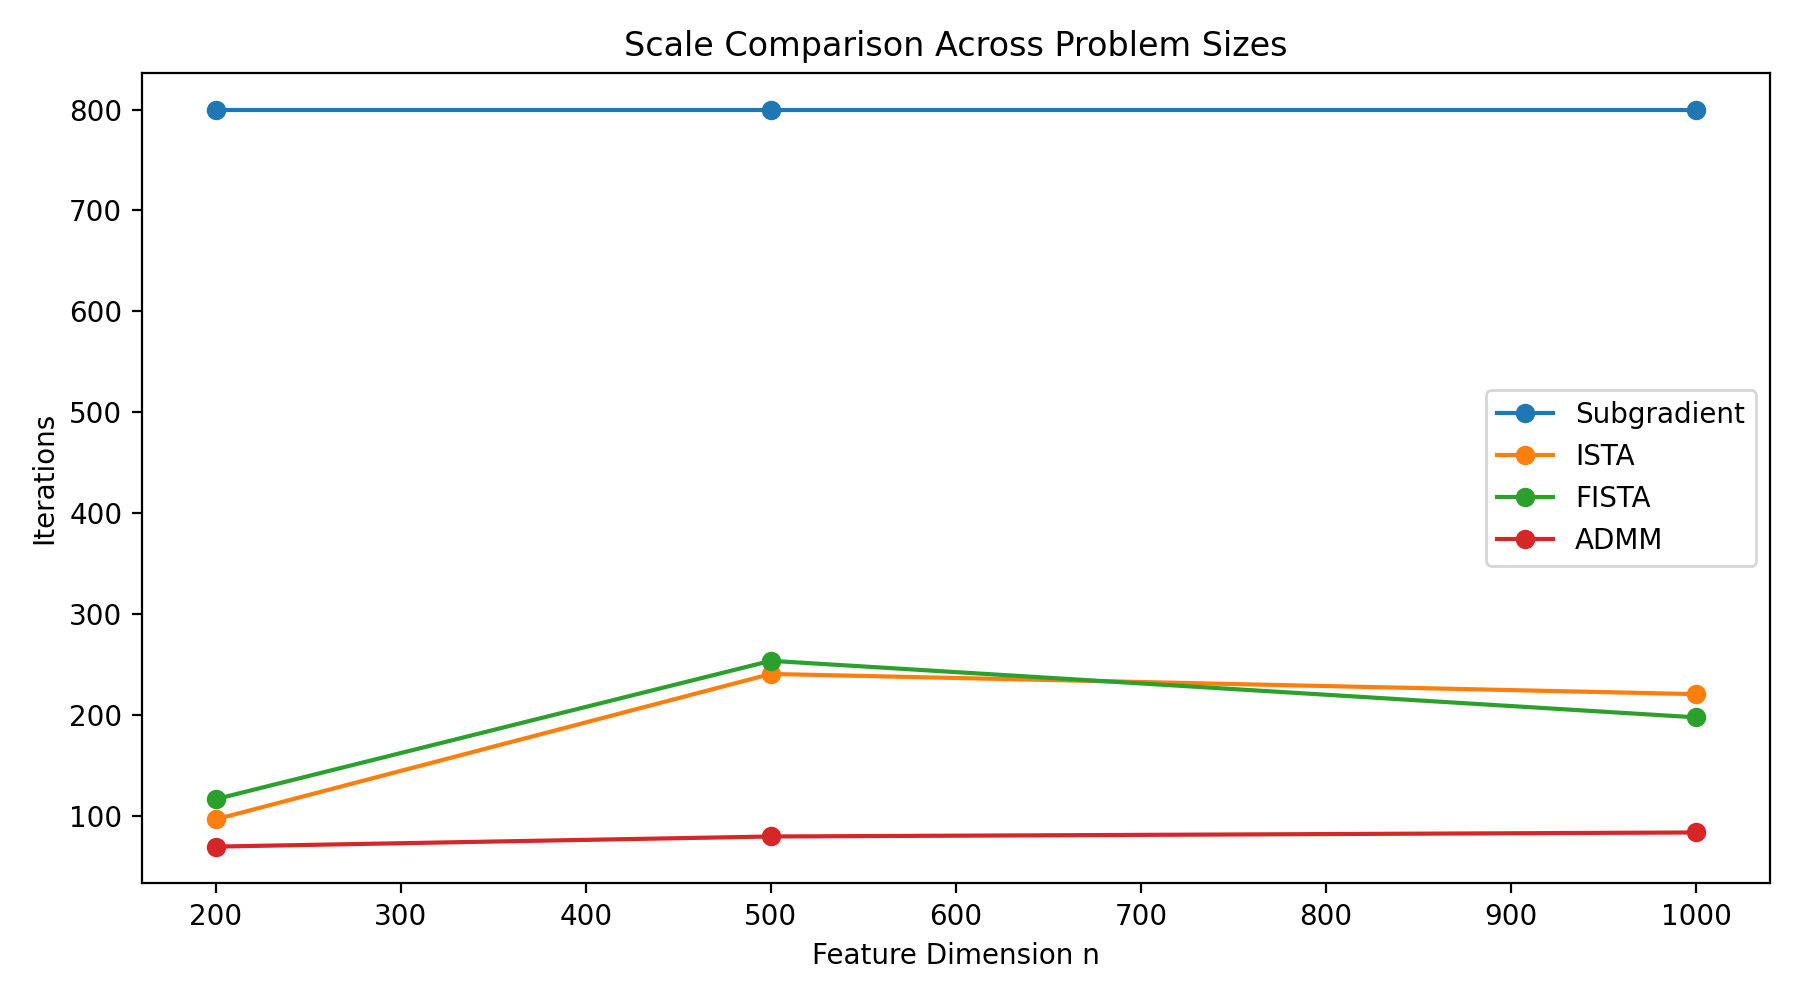
\includegraphics[width=0.72\textwidth]{04_scale_comparison_iterations.png}
    \caption{三档规模实验下各算法迭代次数变化图。随着问题规模从 200 维扩展到 1000 维，ADMM 仍保持较低的迭代成本。}
\end{figure}

\subsection{结果分析}
\begin{enumerate}[label=\arabic*.]
    \item 随着问题维度从 200 增长到 1000，ADMM、ISTA、FISTA 的恢复误差有所上升，这是更高维问题更困难的自然表现；
    \item 在三档规模下，ADMM 与 ISTA/FISTA 的恢复误差几乎一致，说明它并未牺牲解质量；
    \item ADMM 在三档规模下的迭代次数始终较低，分别为 70、80、84，展现出较好的规模适应性；
    \item Subgradient 在所有规模下都表现最差，且始终跑满最大迭代次数。
\end{enumerate}

\subsection{结论}
三档规模实验表明，随着问题规模增大，ADMM 仍然能够在保证解质量的同时保持较低的迭代成本，这进一步支撑了其在高维稀疏恢复问题中的效率优势。

\section{补充实验三：正则化路径可视化（早期扩展）}
\subsection{实验目的}
观察“所有特征系数随 $\lambda$ 变化的路径”，直观展示 Lasso 如何通过增大正则化强度逐步压缩系数。

\subsection{实验设置}
\begin{itemize}[leftmargin=2em]
    \item 合成数据
    \item 求解器：ADMM
    \item $\lambda \in \{0.01, 0.02, 0.05, 0.1, 0.2, 0.5, 1.0\}$
\end{itemize}

\subsection{结果解释}
随着 $\lambda$ 增大，越来越多的特征系数逐渐向 0 收缩，路径图可以清楚展示 Lasso 的稀疏化机制。这项实验已经满足最初方案中的“正则化路径可视化”设想。

\begin{figure}[H]
    \centering
    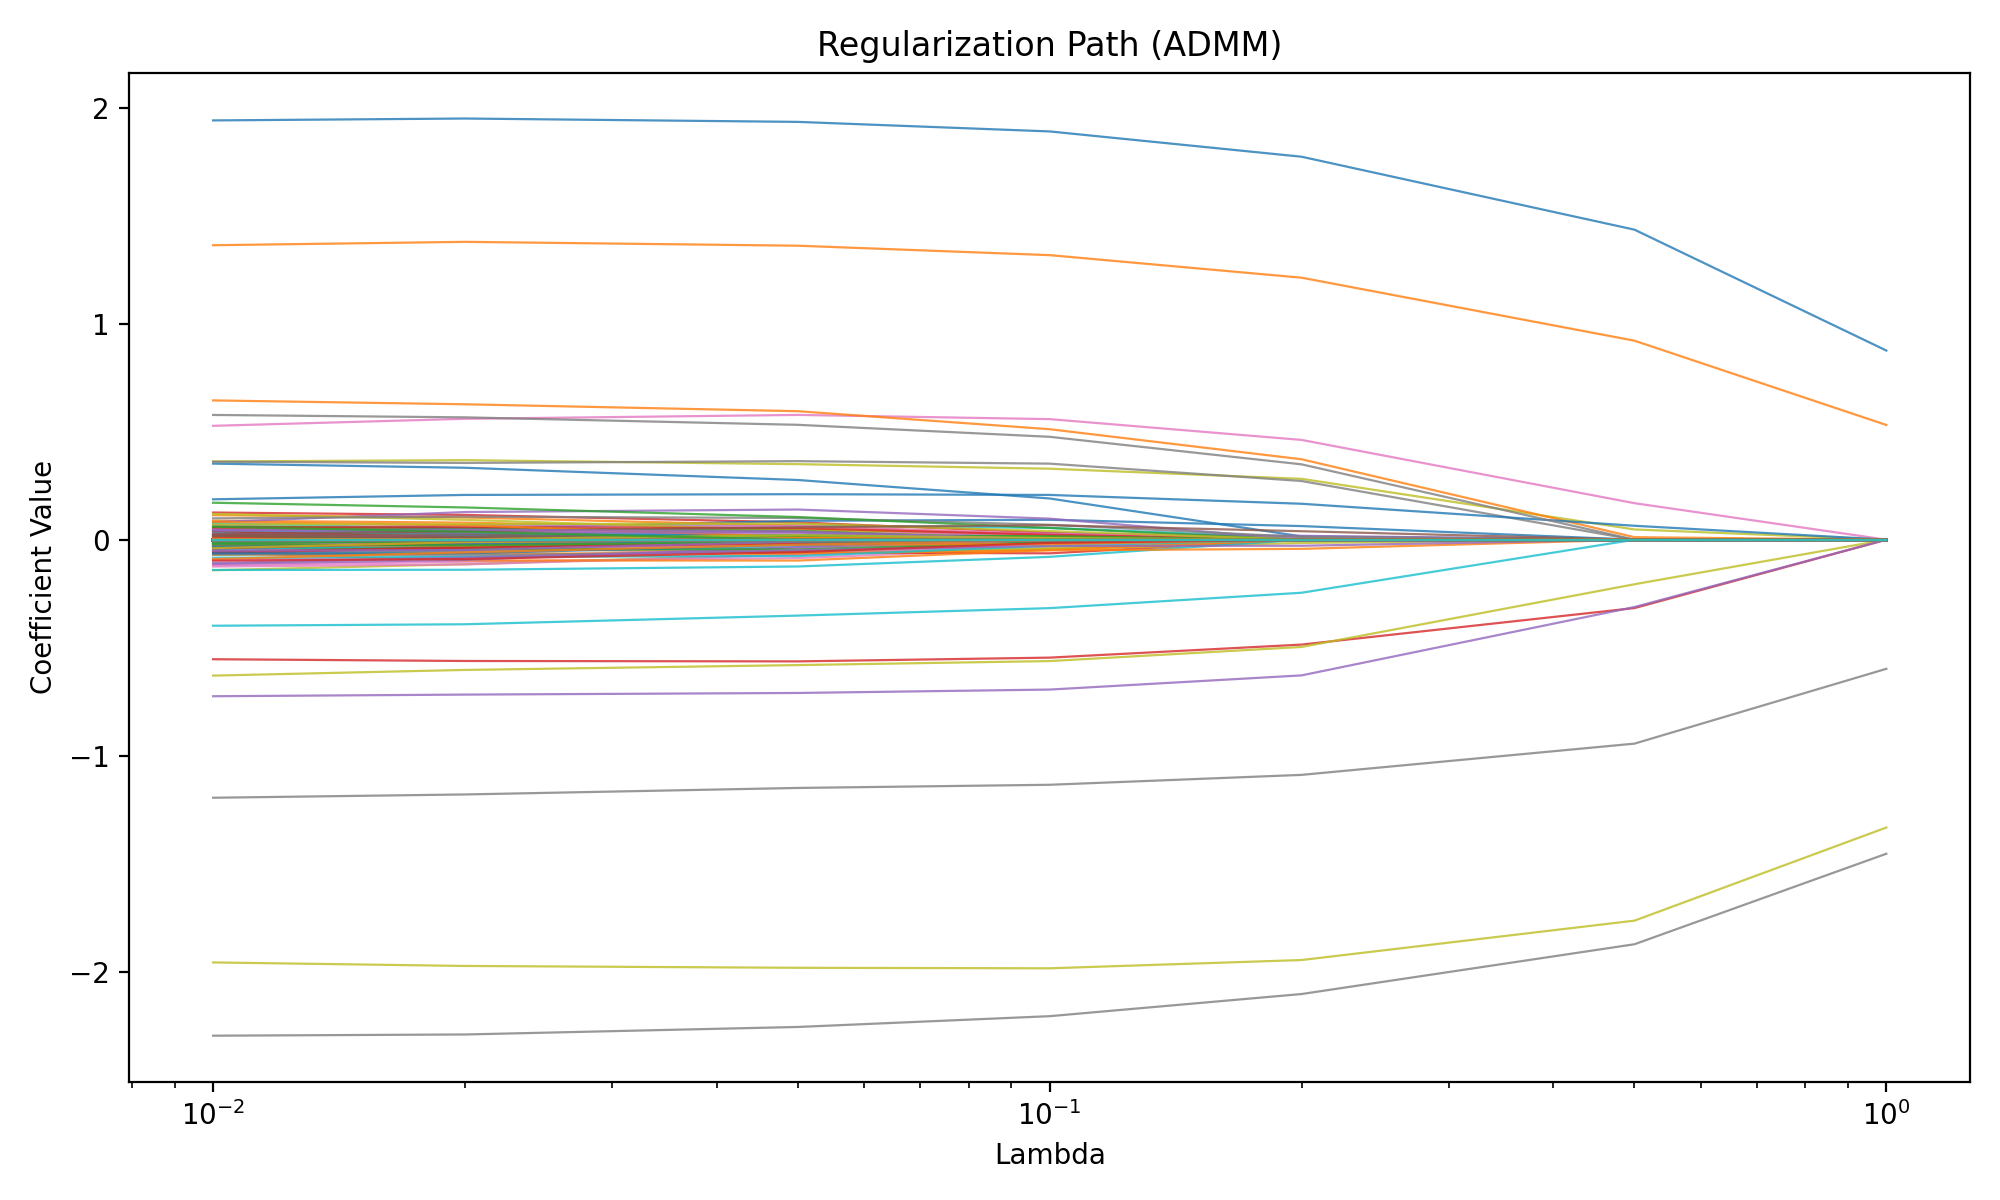
\includegraphics[width=0.86\textwidth]{05_regularization_path_admm.png}
    \caption{ADMM 对应的正则化路径图。随着 $\lambda$ 增大，更多系数逐渐收缩到 0，直观展示了 Lasso 的特征选择与稀疏化机制。}
\end{figure}

\section{补充实验四：相变分析（早期扩展）}
\subsection{初版问题}
最开始，相变分析采用更高维、更严格设置，得到的成功率全部为 0，无法形成有效曲线。

\subsection{相变的含义}
所谓“相变”，是指当噪声水平、观测条件或稀疏度跨过某一区间后，恢复成功率会从较高区间迅速跌落到较低区间的现象。在稀疏恢复问题中，相变常被用来刻画算法对噪声和采样条件的敏感性。因此，本节实验并不是简单画一条成功率曲线，而是希望观察恢复性能是否会随着参数变化出现明显跃迁。

\subsection{改进后的正式设置}
为得到更有解释性的相变趋势，我们采用：
\begin{itemize}[leftmargin=2em]
    \item $m=120$
    \item $n=300$
    \item 稀疏度 $s=10$
    \item $\lambda=0.1$
    \item $\rho=1$
    \item $\sigma \in \{0.00, 0.01, 0.05, 0.10, 0.20\}$
    \item 每个噪声水平重复 10 次
\end{itemize}

\subsection{两种成功标准}
\begin{enumerate}[label=\arabic*.]
    \item \textbf{严格标准（exact）}：恢复出的支撑集与真实支撑集完全一致才算成功；
    \item \textbf{宽松标准（relaxed）}：命中至少 80\% 的真实非零位置即视为成功。
\end{enumerate}

\subsection{严格版结果}
\begin{itemize}[leftmargin=2em]
    \item $\sigma=0.00$ 时成功率约 0.3
    \item $\sigma=0.01$ 时成功率约 0.5
    \item $\sigma \ge 0.05$ 时成功率降为 0
\end{itemize}

\subsection{宽松版结果}
\begin{itemize}[leftmargin=2em]
    \item $\sigma=0.00, 0.01, 0.05, 0.10$ 时成功率接近 1.0
    \item $\sigma=0.20$ 时成功率约 0.9
\end{itemize}

\begin{figure}[H]
    \centering
    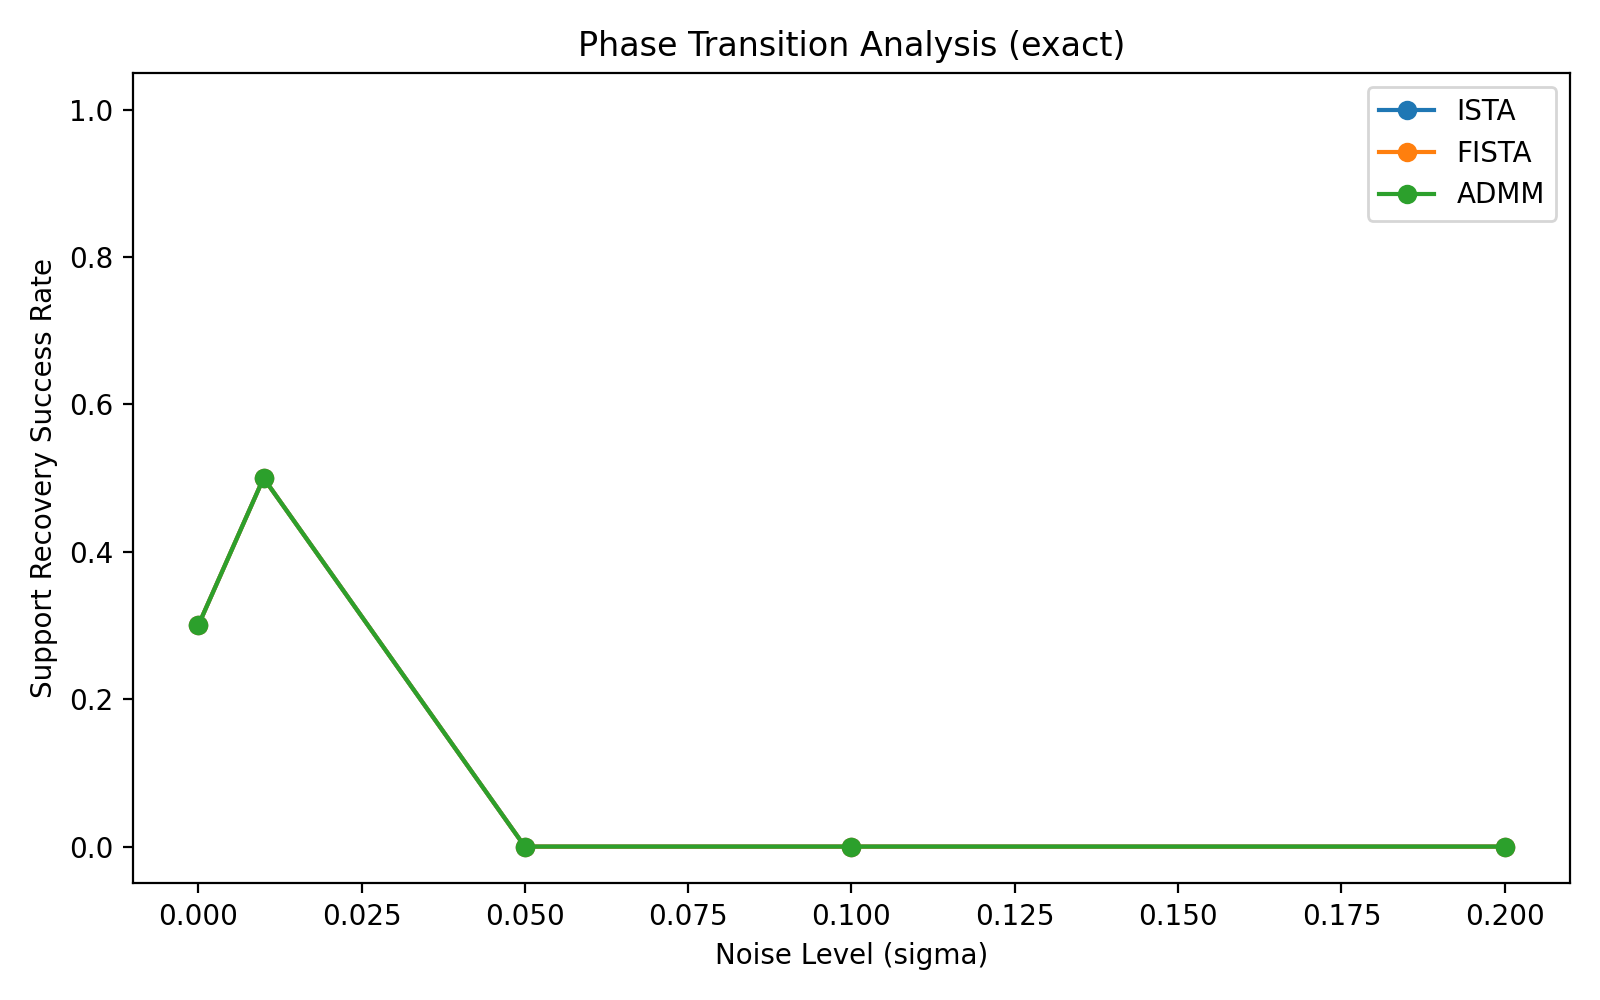
\includegraphics[width=0.47\textwidth]{06_phase_transition_exact_success_rate.png}\hfill
    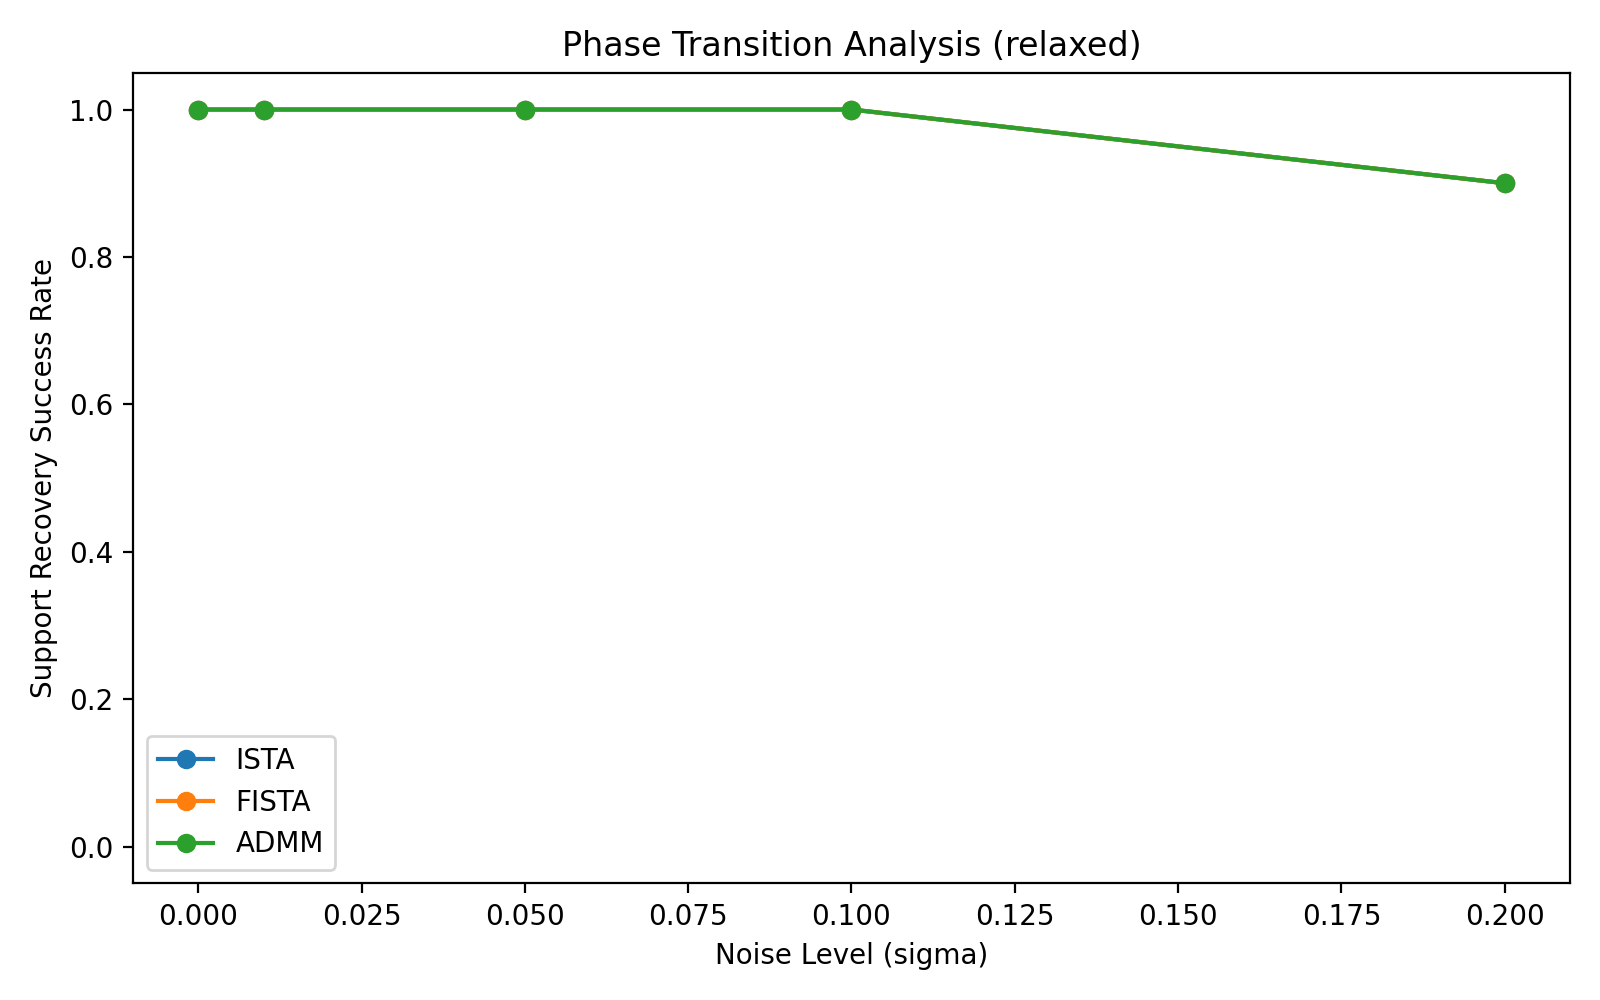
\includegraphics[width=0.47\textwidth]{07_phase_transition_relaxed_success_rate.png}
    \caption{相变分析结果。左图为严格成功标准，右图为宽松成功标准。两种口径都表明：噪声越大，恢复成功率越低。}
\end{figure}

\subsection{结论}
严格标准下，仅低噪声时才有较明显的完全恢复概率；宽松标准下，算法在低到中等噪声下仍能恢复大部分真实非零位置。该实验现已能够支撑“相变分析”的汇报内容，同时也反映出我们对初版不理想实验结果所做的修正。

\section{实验十：真实数据实验}
\subsection{真实数据一：diabetes}
\subsubsection{实验目的}
验证算法在小规模真实回归任务中的预测误差和收敛效率。

\subsubsection{结果特点}
\begin{itemize}[leftmargin=2em]
    \item 四种算法的测试 MSE 均约为 0.475，预测误差接近；
    \item ADMM 仅使用 11 次迭代，明显少于其他算法；
    \item 修正步长后，Subgradient 可以稳定运行。
\end{itemize}

\subsection{真实数据二：wine\_red}
\subsubsection{实验目的}
作为第二个真实回归数据集，验证结果是否在另一个数据集上仍然成立。

\subsubsection{实验设置}
使用 UCI Wine Quality 红酒数据集，目标变量为 \texttt{quality}，其余数值列作为特征。

\subsubsection{结果特点}
\begin{itemize}[leftmargin=2em]
    \item 最终统一重跑采用 $\lambda=0.1$；
    \item 四种算法测试 MSE 均约为 0.599，预测误差非常接近；
    \item ADMM 仅使用 12 次迭代，效率优势清晰；
    \item Subgradient 虽然能运行，但整体效率不如其他方法。
\end{itemize}

\subsection{真实数据三：Communities and Crime}
\subsubsection{实验目的}
将实验扩展到一个更复杂的高维真实回归数据集，用于验证 Lasso 及其优化算法在“存在缺失值、需要清洗、特征维度较高”的实际场景中的表现。

\subsubsection{数据特点}
\begin{itemize}[leftmargin=2em]
    \item 原始数据包含 1994 个样本、128 个属性；
    \item 存在缺失值；
    \item 包含若干 ID/名称类非预测字段；
    \item 目标变量为 \texttt{ViolentCrimesPerPop}。
\end{itemize}

\subsubsection{清洗流程}
为保证可用于回归实验，我们采用了以下清洗流程：
\begin{enumerate}[label=\arabic*.]
    \item 使用 \texttt{communities.names} 恢复列名；
    \item 将 `?` 视为缺失值；
    \item 删除非预测列：\texttt{state, county, community, communityname, fold}；
    \item 删除缺失比例超过 30\% 的特征列；
    \item 对剩余缺失值使用中位数填补；
    \item 划分训练集/测试集，并进行标准化。
\end{enumerate}

清洗后最终保留了 100 个有效特征。

\subsubsection{实验结果与分析}
最终统一重跑采用 $\lambda=0.1$。结果表明：
\begin{itemize}[leftmargin=2em]
    \item ADMM 的测试 MSE 为 0.3113，与 FISTA 的 0.3119 非常接近；
    \item ADMM 保留 99 个非零系数，其他算法约保留 100 个，说明当前参数下稀疏化程度有限；
    \item ADMM 使用 86 次迭代，而 ISTA、FISTA 和 Subgradient 均运行到最大迭代次数 500。
\end{itemize}

\subsubsection{结论}
Communities and Crime 数据集的价值不在于其特征维度一定高于合成数据，而在于它是真实的、带缺失值的、清洗成本较高的复杂回归数据集。最终统一重跑说明：当前 $\lambda=0.1$ 下模型稀疏化程度有限，但 ADMM 仍能以更少迭代达到与 FISTA 接近的预测效果。

\begin{figure}[H]
    \centering
    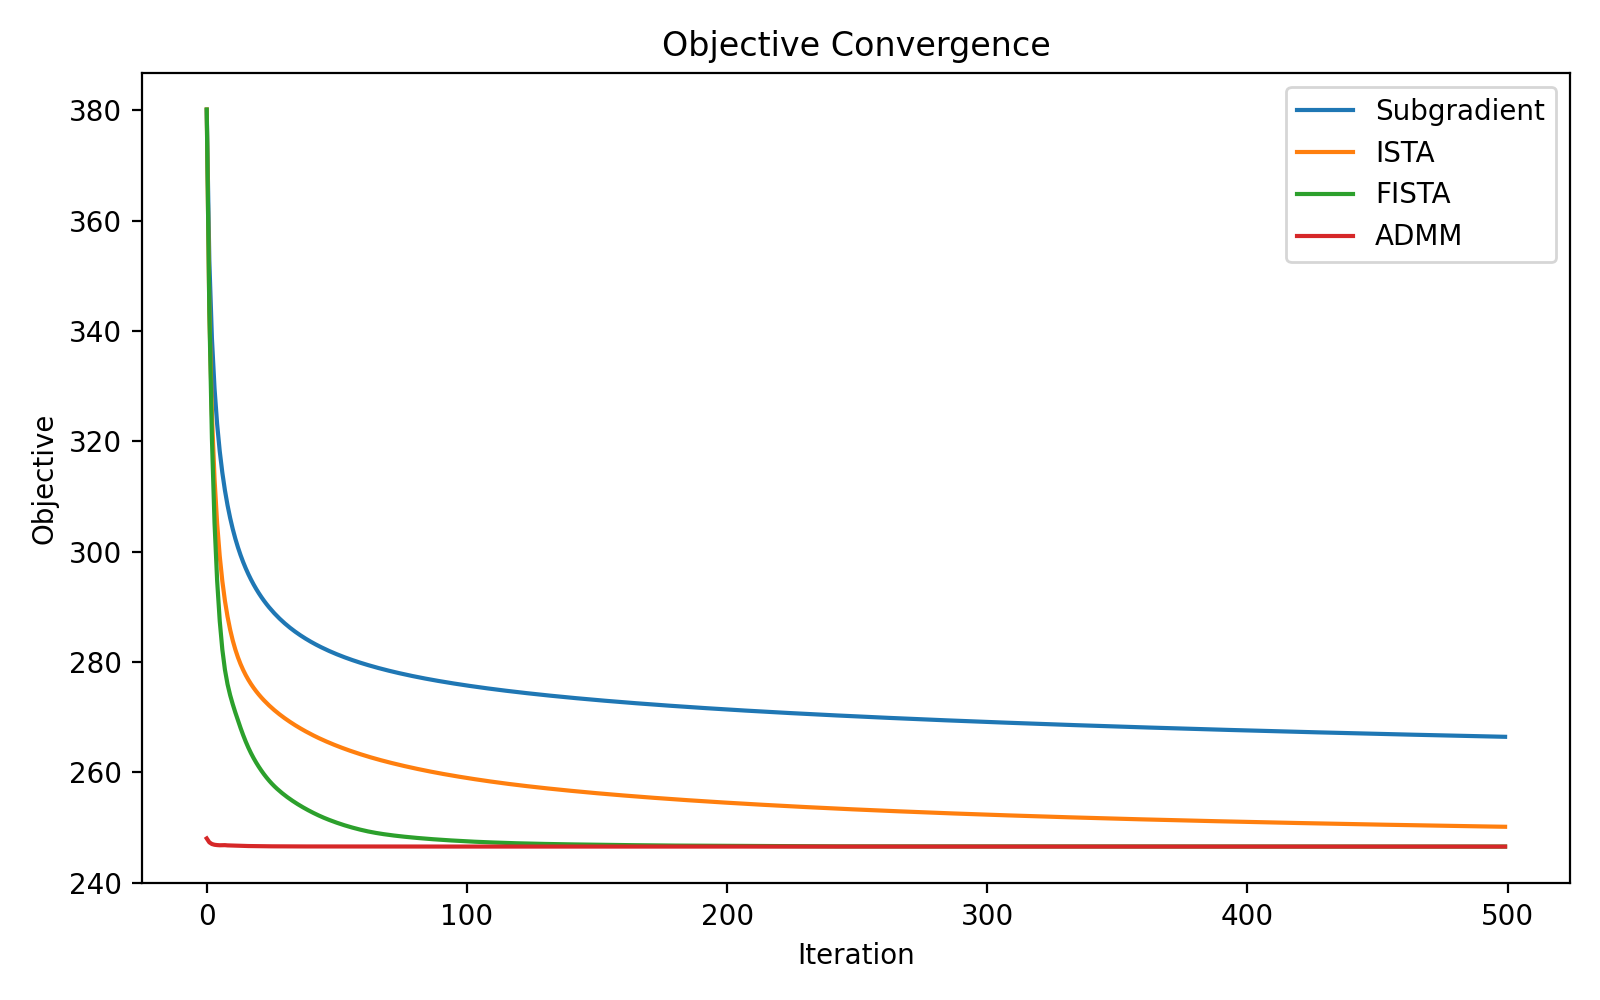
\includegraphics[width=0.78\textwidth]{10_communities_crime_convergence_curve.png}
    \caption{Communities and Crime 数据集上的收敛曲线。该图用于展示复杂真实高维回归场景下各算法的优化过程。}
\end{figure}

\section{实验十一：\texttt{sklearn Lasso} 对照验证}
\subsection{实验目的}
为了增强实验结果的可信度，我们额外引入 \texttt{sklearn.linear\_model.Lasso} 作为参考对照。其作用不是替代我们自己的算法，而是验证自实现的 ADMM、ISTA、FISTA 在代表性场景下是否与成熟库实现具有一致趋势。

\subsection{对照设置}
\begin{itemize}[leftmargin=2em]
    \item \texttt{sklearn Lasso} 的主要作用是“参考验证”，而不是本项目的核心比较对象；
    \item 最终统一重跑在合成数据主实验上进行对照；
    \item \texttt{sklearn} 的目标函数含有样本数归一化，因此使用 $\alpha=\lambda/m$ 与本文目标函数对齐。
\end{itemize}

\subsection{合成数据主实验对照结果}
在最终统一重跑设置下（$m=80,n=200,s=10,\sigma=0.05,\lambda=0.1,\rho=1$），得到：
\begin{itemize}[leftmargin=2em]
    \item FISTA：recovery error = 0.389507，nnz = 17
    \item ADMM：recovery error = 0.389504，nnz = 17
    \item sklearn Lasso：recovery error = 0.389504，nnz = 17
\end{itemize}

这说明在最终统一重跑主实验中，成熟库实现与自实现的结构化方法几乎完全一致。

\subsection{结论}
\texttt{sklearn Lasso} 对照验证表明：本项目中自实现的 ADMM、ISTA、FISTA 与成熟库实现结果趋势一致，从而增强了实验结论的可信度。

\section{当前总体结论}
综合目前已经完成的实验，可以得到以下核心结论：
\begin{enumerate}[label=\arabic*.]
    \item Subgradient 作为 baseline，整体收敛慢、稀疏性差，在合成数据上的表现明显弱于其他三种方法；
    \item ISTA、FISTA、ADMM 都可以有效求解 Lasso，其中 ADMM 在当前实验中迭代次数通常最少；
    \item $\lambda$ 控制拟合误差与稀疏性的平衡；
    \item $\rho$ 主要影响 ADMM 的收敛速度，而不是最终解；
    \item 噪声越大，稀疏恢复越困难；
    \item 多随机种子重复实验表明主结论具有稳定性，不是单次随机实验的偶然结果；
    \item 三档规模实验表明 ADMM 在问题规模增大时仍保持较好的效率优势；
    \item 在真实数据上，结构化方法的预测精度通常接近，但 ADMM 仍具有较强的收敛效率优势；
    \item 在 Communities and Crime 数据集上，当前 $\lambda=0.1$ 下稀疏化程度有限，但 ADMM 仍以更少迭代达到与 FISTA 接近的预测效果；
    \item \texttt{sklearn Lasso} 对照验证表明，自实现结构化方法与成熟库实现结果高度一致，增强了实验可信度；
    \item 正则化路径和相变分析补足了本项目作为 Lasso 优化实验的完整性。
\end{enumerate}

\section{结论与展望}
本文围绕 Lasso 回归中的优化求解问题，系统比较了 Subgradient、ISTA、FISTA 和 ADMM 四种算法，并在合成数据与真实数据上完成了较为完整的实验验证。综合实验结果，可以得到以下结论：
\begin{enumerate}[label=\arabic*.]
    \item 在本文采用的合成数据主实验设置下，ISTA、FISTA 和 ADMM 都能恢复出接近真实稀疏度的解，而 Subgradient 作为直接处理非光滑项的 baseline，表现明显较差。
    \item 在本文采用的数据规模、停止准则与参数设置下，ADMM 在保持与 ISTA/FISTA 接近解质量的同时，通常具有更少的迭代次数，因此表现出较强的效率优势。
    \item 正则化参数 $\lambda$ 决定了拟合精度与稀疏性之间的权衡；较小的 $\lambda$ 更利于减小误差，而较大的 $\lambda$ 更利于恢复稀疏结构。
    \item ADMM 参数 $\rho$ 对最终解影响较小，但对收敛速度影响显著；在本文考察的范围内，$\rho=1$ 表现最佳。
    \item 噪声越大，恢复误差越大，恢复出的解越不稀疏，说明观测噪声会显著削弱对真实稀疏结构的识别能力。
    \item 多随机种子重复实验与三档规模实验说明：本文主结论不仅稳定，而且在更大问题规模下仍然成立。
    \item 在真实数据上，几种结构化方法的预测误差通常比较接近；其中 Communities and Crime 进一步说明，当前参数下模型可能不会自动呈现强稀疏性，但 ADMM 仍具有明显的迭代效率优势。
    \item \texttt{sklearn Lasso} 对照实验表明，在本文所考察的代表性场景下，自实现的 ADMM、ISTA、FISTA 与成熟库结果高度一致，从而增强了实验结论的可信度。
\end{enumerate}

未来如果继续扩展该课题，可以考虑以下方向：
\begin{itemize}[leftmargin=2em]
    \item 对更多真实高维回归数据集进行验证；
    \item 引入更系统的超参数选择方法，如交叉验证；
    \item 将 Lasso 扩展到 Elastic Net、Group Lasso 等更复杂的稀疏建模任务；
    \item 从理论角度补充不同算法的收敛性质与复杂度分析。
\end{itemize}

\end{document}
